\documentclass{article}
\usepackage{amsmath}
\usepackage{bbm}
\usepackage{amssymb}
%\usepackage[ruled,vlined]{algorithm2e}
\usepackage{algorithm,algpseudocode}
\usepackage{xcolor}
\usepackage{hyperref}
\hypersetup{
    colorlinks=true,
    linkcolor=blue,
    filecolor=magenta,      
    urlcolor=cyan,
    pdftitle={Overleaf Example},
    pdfpagemode=FullScreen,
    }
    
\usepackage[shortlabels]{enumitem}
\usepackage{bm}
\usepackage{graphicx}
\usepackage{dirtytalk}
\usepackage{subcaption}

\usepackage{xspace}
\usepackage{tcolorbox}
\tcbuselibrary{listings}
\newtcblisting{foo}{
  listing only,
  nobeforeafter,
  after={\xspace},
  hbox,
  tcbox raise base,
  fontupper=\ttfamily,
  colback=lightgray,
  colframe=lightgray,
  size=fbox
  }

% Declare Operators
\newcommand{\weight}{w}
\newcommand{\bias}{b}
\newcommand{\slack}{\xi}
\newcommand{\dual}{v}
\newcommand{\xv}{\mathbf{x}}
\newcommand{\const}{C}
\newcommand{\margin}{M}
\newcommand{\kernel}{K}
\newcommand{\kernelmap}{\phi}
\newcommand{\half}{\frac{1}{2}}
\newcommand{\param}{\gamma}
\newcommand{\st}{\mathop{\mathrm{subject\,\,to}}}

\usepackage[utf8]{inputenc}

\title{10-715 Fall 2022 Homeworks}

\begin{document}

\begin{center}
{\Large CMU 10-715: Homework 8}\\
Online Learning and Q Learning \\
{\bf DUE: Dec. 12, 2022, 11:59 PM}.\\
\end{center}


\textbf{\large Instructions}:
\begin{itemize}
    \item \textbf{Collaboration policy:} Collaboration on solving the homework is allowed, after you have thought about the problems on your own. It is also OK to get clarification (but not solutions) from books, again after you have thought about the problems on your own. Please don’t search for answers on the web, previous years’ homeworks, etc. (please ask the TAs if you are not sure if you can use a particular reference). There are two requirements: first, cite your collaborators fully and completely (e.g., ``Alice explained to me what is asked in Question 4.3''). Second, write your solution \emph{independently}: close the book and all of your notes, and send collaborators out of the room, so that the solution comes from you only. 
    \item \textbf{Submitting your work:} Assignments should be submitted as PDFs using Gradescope unless explicitly stated otherwise. Each derivation/proof should be completed on a separate page. Submissions can be handwritten, but should be labeled and clearly legible. Else, submission can be written in LaTeX.
    
    \item \textbf{Late days:} For each homework you get three late days to be used only when anything urgent comes up. No points will be deducted for using these late days. We will consider an honor system where we will rely on you to use the late days appropriately.
    

\end{itemize}

% Q1 - Online Learning
\newpage 
\section{[50 pts] Online Learning} 

We want to predict if the stock market will go up or down. On day $t$, we observe the actual outcome $y_t\in \{ -1, 1\}$. Assume we have $N$ experts who would vote positive ($+1$) or negative ($-1$) on each day $t$. 
Consider the following online learning algorithm for this binary prediction problem:
\vspace{5mm}

\begin{algorithm}[H]
\begin{algorithmic}

%\SetAlgoLined
\State \textbf{Input:} Pool of $d$ experts: $S=\{1,\cdots, d\}$, number of days: $T$, Hyperparameter $\epsilon$
%\step 
\State Initialize $w = (1, 1, \ldots, 1) \in \mathbb{R}^d$ 
\vspace{2mm}
\For{$t\gets 1$ \textbf{to} $T$}
    \State (Randomly) Choose an expert $i \in [d]$ with probability $w_i/(\sum_j w_j)$ 
    \State Make a prediction based on chosen expert 
    \State Update the weights for every wrong expert $j \in [d]$ as follows: 
    \begin{align*} w_j \gets (1 - \epsilon) w_j \,. \end{align*}
\EndFor    
\caption{Randomized weighted majority algorithm}

\end{algorithmic}
\end{algorithm}
\vspace{3mm}

\begin{itemize}
	\item Implement the randomized weighted majority algorithm and run the algorithm on the dataset \emph{online\_data.csv}. For this dataset, we have $d =10$ and $T = 10k$. The goal here is to predict as well as the best expert does in the hindsight. Append your code to your PDF submission. \\
	\item Compute your regret for the values of epsilon in the following set: 
			$$\mathcal{E} = \{0.05, 0.1, 0.3, 0.5, 0.7, 0.9, 0.95\}\,.$$ 
			For each epsilon $\epsilon \in \mathcal{E}$, run 3 different seeds (100, 200, 300), and plot the mean  as well as mean $\pm$ standard deviation of the regret versus epsilon. Compare your results with a simple baseline where you choose the best expert so far. Add this as a baseline in the plot. Note that this baseline doesn't depend on epsilon and hence, we expect a horizontal line for the baseline.   Summarize your observations in 2-3 sentences. 

\end{itemize}


% Q2 - Q Learning
\newpage
\section{[50 pts] Q Learning}

In this question you will implement the Q Learning algorithm.

\begin{algorithm}
\caption{Q Learning}\label{alg:cap}
\begin{algorithmic}
\Require $\alpha, \epsilon, \gamma, ENV$
\While{$episode \leq MAX\_ITERATIONS$}
\State Reset ENV and get initial state $s$
\While{$episode$ not done}
    \State Sample action $a$\Comment{according to $\epsilon$-greedy strategy}
    \State Get new state $s'$, reward $r$
    \State Update $Q[s, a] = (1-\alpha)Q[s, a] + \alpha(r + \gamma \max_{a'} Q[s', a'])$
    \State update State $s$ to new state $s'$
\EndWhile
\EndWhile\\
\Return Q
\end{algorithmic}
\end{algorithm}

\noindent
We have provided the starter code in \emph{qlearning\_starter.py}, where you will be using FrozenLake environment from gym. To install gym, simply run \begin{foo}pip install gym \end{foo} 
or \begin{foo}pip3 install gym\end{foo}. 

For more details about gym, please refer to \hyperlink{https://github.com/openai/gym}{https://github.com/openai/gym}. For the following questions, the start code has outlined \emph{TODO} blocks. Don't forget to append your code to your PDF submission.

\begin{enumerate}[(a)]
    \item (20 points) Run the Q Learning algorithm using the default hyperparameters given ($\alpha=0.8, \gamma=0.9, \epsilon=0.7$). You'll also need to write the $\epsilon-$greedy algorithm in order to sample the action at each time step.
    
    \item (30 points) Evaluate the environment using an $\epsilon-$greedy strategy. 
    		\begin{itemize}
    			\item For each $\epsilon$ in $\{0, 0.25, 0.5\}$, report an episode of the game (see example below). You can use $env.render()$ and plot the whole game trajectory. 
    			\item Describe the difference among the three episodes, and provide your interpretation. \\
    		\end{itemize}
    		
    
    \newpage
    
    \begin{figure}[H]
    	\centering
	    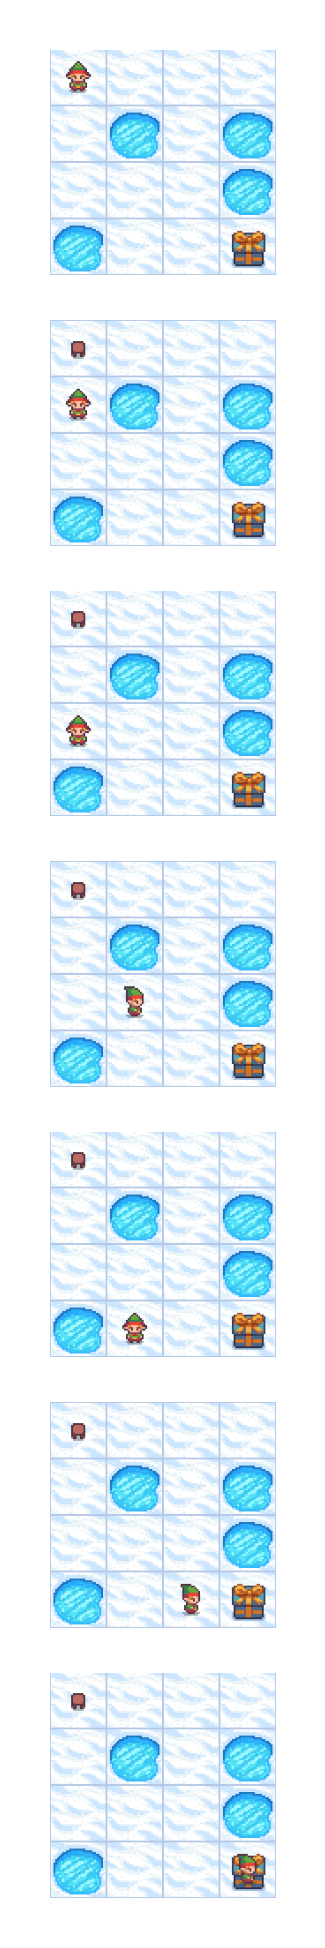
\includegraphics[width=0.25\linewidth]{./example.png}
    	\caption{Example of an episode}
	    \label{fig:q2}
	\end{figure}

    
    
\end{enumerate}

\end{document}